










\chapter*{Pesquisa sobre a Importância de se utilizar teste automatizados}
\label{apendice:1}

\par Nesta apêndice são mostradas as perguntas que foram feitas através do google \textit{forms}, para obter dados relevantes sobre, se os desenvolvedores utilizam testes automatizados no processo de desenvolvimento do \textit{software}.
\par Na Figura 57 estão todas as perguntas que foram feitas.

\begin{figure}[!htb]
    \caption[Perguntas sobre a importância de se utilizar teste automatizados ]{Perguntas sobre a importância de se utilizar teste automatizados.
    
     \centering
     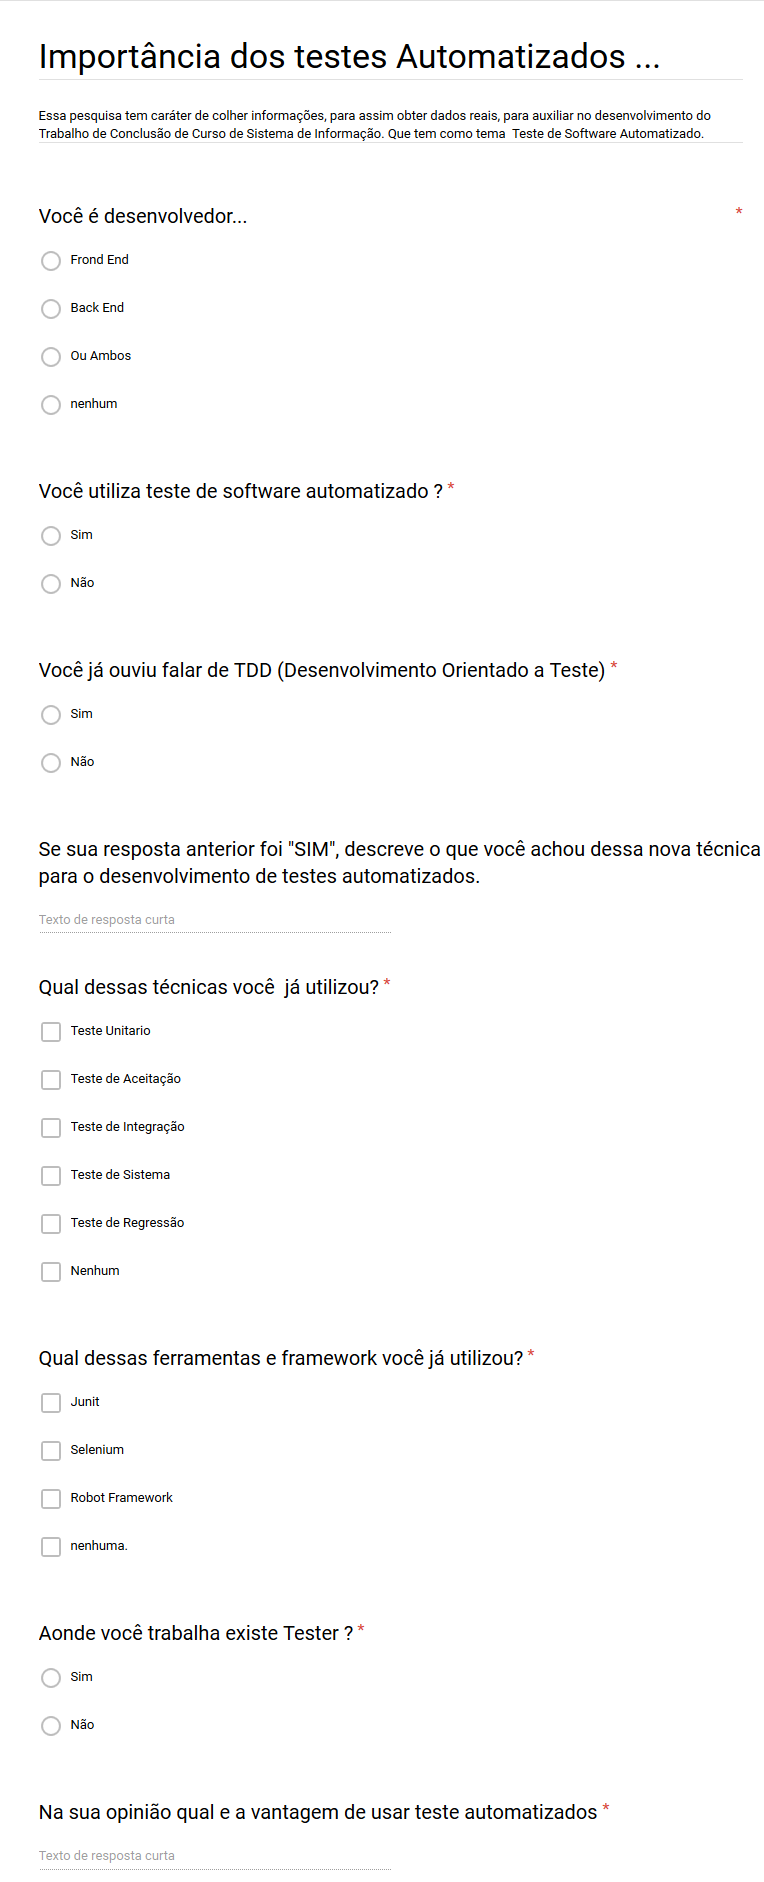
\includegraphics[width=12cm,height=25cm]{imagens/perg4.PNG}
     
     \textbf{Fonte: } Elaborado pelos autores.}
     \label{fig:Perguntas sobre a importância de se utilizar teste automatizados}
\end{figure}

\begin{comment}

Na Figura 55, 56 e 57 é ilustrada a primeira pergunta da pesquisa.

\begin{figure}[!htb]
    \caption[Perguntas sobre a importância de se utilizar teste automatizados ]{Perguntas sobre a importância de se utilizar teste automatizados.
    
     \centering
     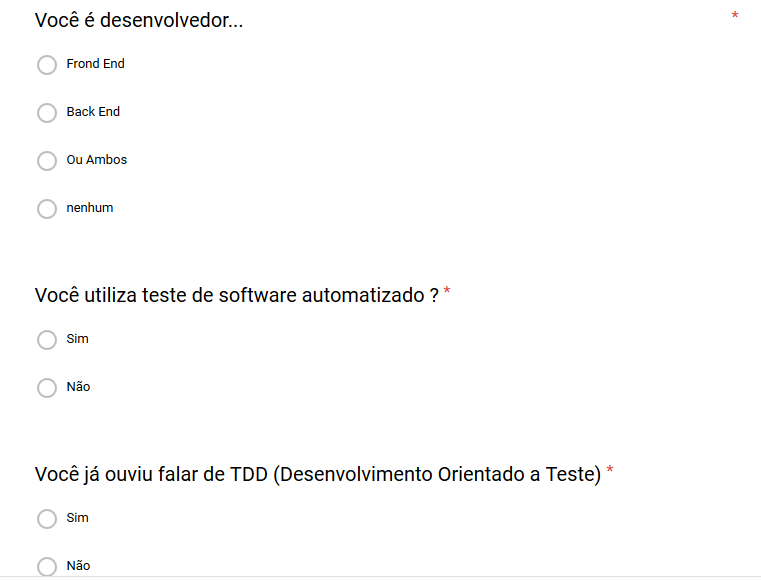
\includegraphics[width=18cm,height=8cm]{imagens/perg1.PNG}
     
     \textbf{Fonte: } Elaborado pelos autores.}
     \label{fig:Perguntas sobre a importância de se utilizar teste automatizados}
\end{figure}

\begin{figure}[!htb]
    \caption[Perguntas sobre a importância de se utilizar teste automatizados ]{Perguntas sobre a importância de se utilizar teste automatizados.
    
     \centering
     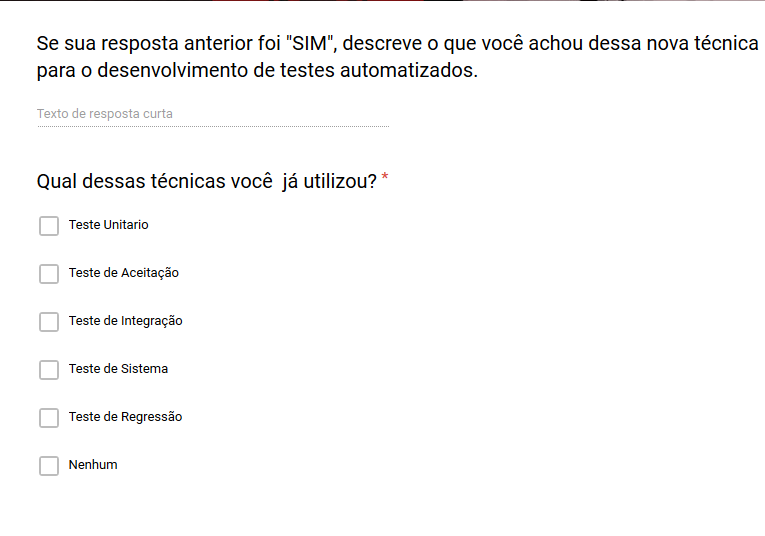
\includegraphics[width=18cm,height=8cm]{imagens/perg2.PNG}
     
     \textbf{Fonte: } Elaborado pelos autores.}
     \label{fig:Perguntas sobre a importância de se utilizar teste automatizados}
\end{figure}

\begin{figure}[!htb]
    \caption[Perguntas sobre a importância de se utilizar teste automatizados ]{Perguntas sobre a importância de se utilizar teste automatizados.
    
     \centering
     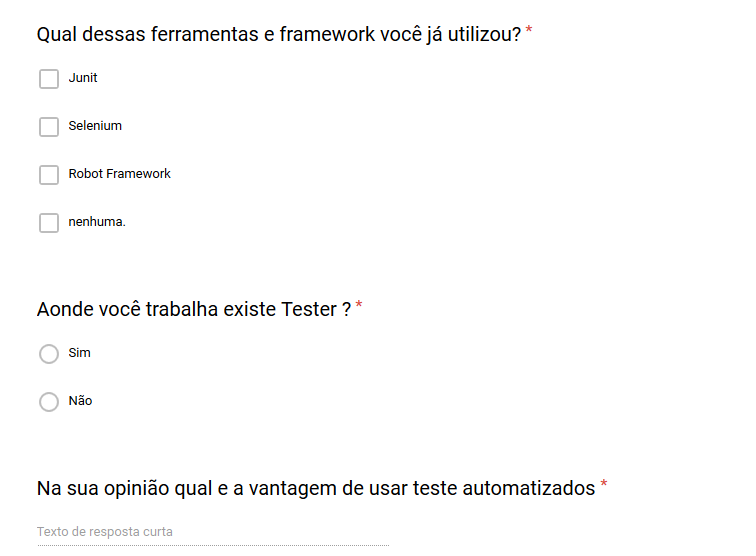
\includegraphics[width=18cm,height=20cm]{imagens/perg3.PNG}
     
     \textbf{Fonte: } Elaborado pelos autores.}
     \label{fig:Perguntas sobre a importância de se utilizar teste automatizados}
\end{figure}

\end{comment}



\begin{comment}

\captionsetup[figure]{list=no}
\begin{figure}[h!]
 \centerline{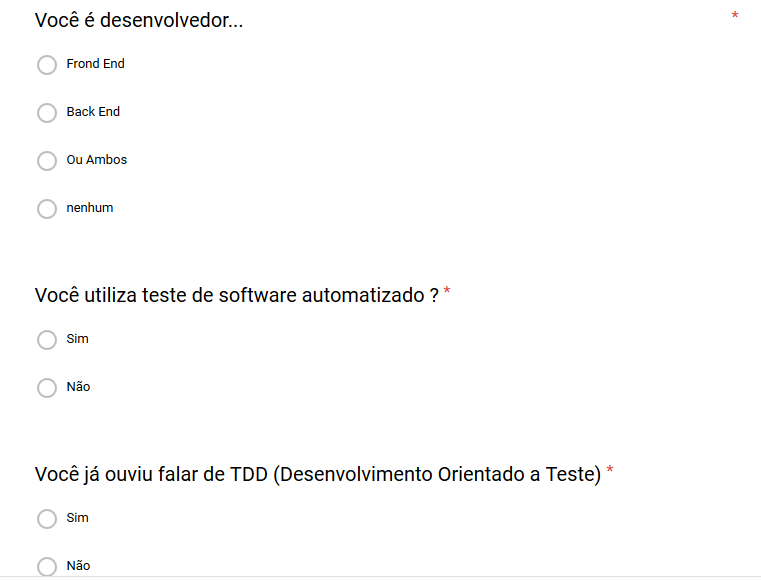
\includegraphics[scale=0.5]{./imagens/perg1.PNG}}
 \caption[Outra imagem.]
           {Outra imagem. \textbf{Fonte:} Elaborado pelos autores}
  \label{fig:ap1:identificador}
\end{figure}

\par Após a seleção do tipo de projeto \ldots
 ~\ref{apendice:1}.
\end{comment}